\section{Kompression}\label{sec:compression}

\subsection{Motivation}

Unabhängig davon, ob man eine Ausstellung in einem Museum gestaltet oder eine Webseite erstellt, lässt sich fast jede für Besucher oder Benutzer konzipierte Darstellung durch den Einsatz von Bildern aufwerten. Dieses lässt sich durch den Einsatz von 3D-Modellen, mit welchen der Benutzer durch Drehen, Zoomen, etc. interagieren kann, noch deutlich steigern. Abgesehen davon, dass dies in einer Ausstellung nur durch den Einsatz von Rechnern, wie beispielsweise von Tablets, möglich ist, sind damit jedoch einige technische Herausforderungen verbunden.

Einerseits erwartet der Benutzer ein möglichst realistisches Erlebnis, was nur durch hochaufgelöste 3D-Modelle und den damit einhergehenden großen Datenmengen möglich ist. Dennoch soll das Modell möglichst ohne Latenz angezeigt werden und flüssige Interaktion erlauben. Soll die Darstellung darüber hinaus auf einem mobilen Endgerät des Benutzers, wie beispielsweise einem Smartphone, stattfinden, das einerseits nur eingeschränkte Rechenkapazität bietet und auf das andererseits die gesamten Daten für jeden Benutzer separat übertragen werden müssen, entsteht hier ein Gegensatz, für den ein geeigneter Kompromis zu finden ist.

Dieser Kompromis besteht darin, die 3D"=Modelle nicht in der höchsten verfügbaren Auflösung dem Benutzer darzustellen, sondern in einer dem Anwendungsfall und dem Endgerät angemessenen Größe. Beispielsweise ist für eine ansprechende Anzeige auf einem Smartphone"=Bildschirm eine geringere Auflösung notwendig als auf der Workstation eines Museumsmitarbeiters mit entsprechend großem Bildschirm, die auch dementsprechend leistungsfähig ist, und über welche dieser Mitarbeiter das angezeigte Objekt erforschen möchte. Aus diesem Grund ist es sinnvoll, die gespeicherten 3D"=Modelle in verschiedenen Auflösungen in der Medien-Datenbank bereit zu halten, weshalb diese in der Regel beim Hochladen in die Datenbank automatisch komprimiert werden.

Die eben beschriebene Problematik tritt nicht nur bei 3D"=Modellen auf, sondern auch bei herkömmlichen zweidimensionalen Bildern. Da auch solche Medien in der Medien"=Datenbank gespeichert werden sollen, sind auch Bilddateien zu komprimieren, was sich sehr einfach durch das Verringern der Auflösung bewerkstelligen lässt. Von jedem hochgeladenen Bild werden also komprimierte Versionen in verschiedenen Auflösungsstufen erstellt, auf welche anschließend zugegriffen werden kann.

In diesem Kapitel wird nach einer kurzen Erläuterung der theoretischen Grundlagen auf die an die ViSIT"=Medien"=Datenbank angebundene Kompressions"=Komponente und deren Voraussetzungen, ihre Funktionsweise, die Installation und die Bedienung, die über eine Web-Oberfläche erfolgt, eingegangen. Außerdem werden die zur Verfügung stehenden Konfigurationsoptionen eingehend erläutert. Abschließend wird die Schnittstelle (API), über welche die Kompressions"=Komponente unabhängig von der dafür verfügbaren Web-Oberfläche oder der ViSIT"=Medien"=Datenbank angesprochen werden kann, spezifiziert.

\subsection{Grundlagen}

Bei 3D-Modellen gilt es grundsätzlich zwischen der Geometrie, durch welche die Form der Oberfläche eines Objekts beschrieben wird, und der Textur, durch welche die Färbung der Oberfläche ausgedrückt wird, zu unterscheiden. Während die Geometrie obligatorisch für ein 3D-Modell ist, muss nicht zwangsläufig eine Textur existieren. Nicht jedes Digitalisierungsverfahren ist in der Lage, Texturdaten zu erfassen, so beispielsweise ein Laserscanner. Im Folgenden werden Aufbau und Kompression dieser beiden Bestandteile eines 3D-Modells behandelt.

\subsubsection{Geometrie von 3D-Modellen}
\label{schlenke:chp:fundamentalsGeometry}

Herkömmliche 3D"=Modelle, die ausschließlich die Oberfläche eines Objekts und nicht dessen Inneres beschreiben, bestehen aus mehreren Punkten im dreidimensionalen Raum, die \emph{Vertices} genannt werden. Diese Punkte werden zu Flächen, den sogenannten \emph{Faces} verbunden, wobei es sich hier in vielen Fällen um Dreiecke handelt. Die Anzahl der Ecken eines Faces wird als dessen \emph{Ordnung} bezeichnet. Die Kanten dieser Flächen, die Verbindungen zwischen zwei Vertices darstellen, werden \emph{Edges} genannt. Die Gesamtheit aller Vertices und Faces eines 3D"=Modells wird auch als \emph{Mesh} bezeichnet. Die soeben genannten Begriffe werden in \autoref{schlenke:fig:fundamentals:geo} grafisch dargestellt.

\begin{figure}
\centering
\subfloat[Vertex]{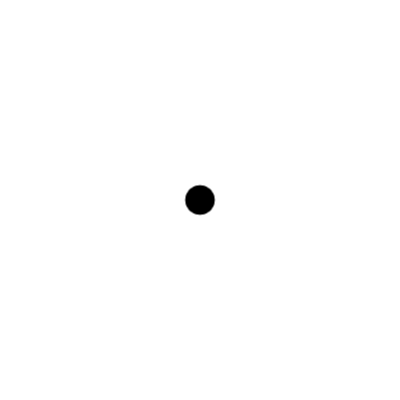
\includegraphics[width=0.25\textwidth]{Figures/schlenker/fundamentals/basicVertex.png}}
\qquad
\subfloat[Edge]{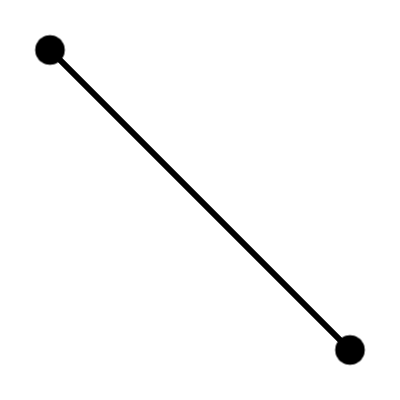
\includegraphics[width=0.25\textwidth]{Figures/schlenker/fundamentals/basicEdge.png}}
\qquad
\subfloat[Face]{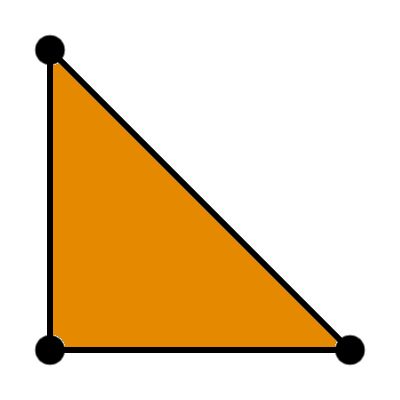
\includegraphics[width=0.25\textwidth]{Figures/schlenker/fundamentals/basicFace.png}}\\
\subfloat[Mesh]{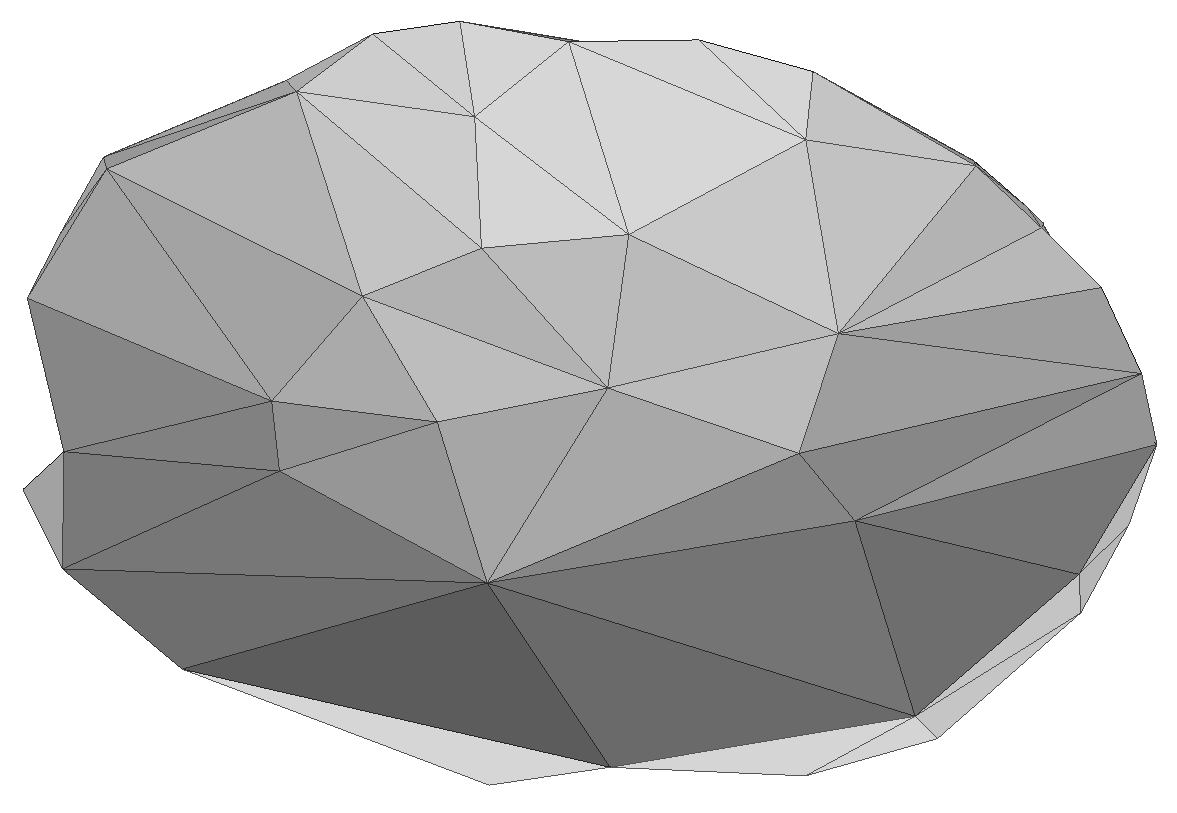
\includegraphics[width=0.70\textwidth]{Figures/schlenker/fundamentals/basicMesh.png}}
\caption{Grundlegende Elemente der Geometrie eines 3D-Modells}
\label{schlenke:fig:fundamentals:geo}
\end{figure}

Während bei einfachen Dateiformaten, wie beispielsweise dem STL-Format\footnote{\url{http://www.fabbers.com/tech/STL_Format}}, für jedes Face die Koordinaten eines jeden Eckpunkts separat gespeichert werden, wird die dadurch verursachte Redundanz zum Beispiel bei OBJ-Dateien\footnote{\url{http://www.martinreddy.net/gfx/3d/OBJ.spec}} vermieden, indem zunächst alle Vertices in Form der Koordinaten einmalig angegeben werden und anschließend bei der Definition der Faces auf diese Vertexdefinition indexbasiert zugegriffen wird.

Bei Meshes, die ein reales Objekt beschreiben, sollte dieser möglichst einer orientierbaren stetigen zweidimensionalen Mannigfaltigkeit, die in den dreidimensionalen Raum eingebettet ist, entsprechen \cite[S.~3]{botsch2010}. Dies hat zur Folge, dass für jeden Punkt im Raum eindeutig entschieden werden kann, ob er im Inneren oder im Äußeren des Objekts liegt. Dies impliziert beispielsweise, dass kein Edge Teil von mehr als zwei Faces sein kann. Jedoch sind auch an die Vertices bestimmte Bedingungen zu stellen, wobei für Details auf \cite[S.~11f]{botsch2010} verwiesen wird.

\subsubsection{Textur von 3D-Modellen}

Die Textur eines 3D"=Modells beschreibt dessen Färbung der Oberfläche, wodurch ihr eine äußerst wichtige Bedeutung für das visuelle Erlebnis beim Betrachten des Modells zukommt. Sie wird in der Regel getrennt von den eigentlichen Geometriedaten in einer separaten Bild"=Datei gespeichert. Für jedes Face wird dann durch die sogenannten \emph{Texturkoordinaten} festgelegt, welcher Ausschnitt des Textur-Bildes auf diesem Dreieck angezeigt wird. Pro Face werden also für jeden Eckpunkt zwei Werte gespeichert, durch welche eine eindeutige Position im Bild definiert wird. Da in der Regel bei den meisten Vertices alle angrenzenden Faces die gleichen Texturkoordinaten verwenden, wird dieses Paar von Werten beispielsweise bei OBJ-Dateien nur einmal gespeichert, worauf anschließend bei der Beschreibung der Faces indexbasiert zugegriffen wird.

Manchem Leser stellt sich hier die Frage, ob generell die Verwendung von einem Paar Texturkoordinaten pro Vertex, welches dann für alle angrenzenden Faces verwendet wird, nicht ausreichend wäre. Hier spielt jedoch die Geometrie des 3D"=Modells, genauer deren \emph{Topologie}, eine wichtige Rolle. Entspricht diese einer (verzerrten) Ebene, so wäre diese Vereinfachung in der Tat ausreichend. Betrachtet man aber beispielsweise eine Kugel, so lässt sich das zweidimensionale Bild nicht über die Kugel legen, ohne dass eine Kante entsteht, an welcher mindestens zwei Ränder des Bildes aneinandergrenzen. Genau entlang dieser Linie, dem sogenannten \emph{Texture Seam}, befinden sich dann die Vertices, für welche je nach angrenzendem Face verschiedene Texturkoordinaten verwendet werden müssen. Unabhängig von der soeben dargelegten Notwendigkeit dieser Texture Seams lässt sich durch eine sinnvolle Unterteilung der Textur auch die Qualität erhöhen, indem für alle Bereiche des 3D"=Modells eine ähnliche Auflösung verwendet wird und durch starke Streckungen oder Stauchungen verursachte Verzerrungen der Textur auf dem Modell minimiert werden.

\subsubsection{Kompression der Geometrie}
\label{schlenke:chp:fundamentals:geocomp}

Eine der wichtigsten Herangehensweisen zur Kompression von 3D"=Modellen ist die Reduktion von Vertices und damit einhergehend die Verringerung der Anzahl an Faces. Ausgehend von einem hoch aufgelösten Modell mit einer hohen Anzahl an Vertices ist die auf den ersten Blick einfachste Vorgehensweise das Entfernen eines möglichst unwichtigen Vertices. Das dadurch entstehende Loch im Mesh muss anschließend geschlossen werden. Dadurch entsteht jedoch im Allgemeinen ein Face mit einer höheren Ordnung, was oft unerwünscht ist. In diesem Fall muss das entstehende Loch mit Dreiecken gefüllt werden, wofür es keine eindeutige und daher auch unterschiedlich gute Lösungen gibt. Stattdessen verwenden viele Kompressionsverfahren, wie auch der in dieser Kompressions-Komponente verwendete Algorithmus, sogenannte \emph{Edge-Collapse}-/\emph{Half-Edge-Collapse}-Operationen.

Bei einer solchen Edge-Collapse-Operation, wie sie in Abbildung \ref{schlenke:fig:fundamentals:edgecollapse} dargestellt ist, werden zwei durch ein Edge verbundene Vertices zu einem neuen Vertex verschmolzen. Dabei degenerieren die an dieses Edge angrenzende Faces und werden entfernt. Zusätzlich lassen sich neben dem kontrahierten Edge noch weitere Edges entfernen. Entspricht der Mesh lokal einer Mannigfaltigkeit, werden durch eine Edge-Collapse-Operation also zwei Faces, drei Edges und ein Vertex entfernt. Vor dem Durchführen einer derartigen Operation muss jedoch überprüft werden, ob die in \cite[S.~118f]{botsch2010} erläuterte \emph{Link Condition} erfüllt ist, da andernfalls die Topologie des Meshes durch die Operation verändert werden kann. Entspricht der neue Vertex einem der beiden ursprünglichen Vertices, so spricht man von einem Half-Edge-Collapse.

\begin{figure}
\centering
\subfloat[Situation vor der Operation]{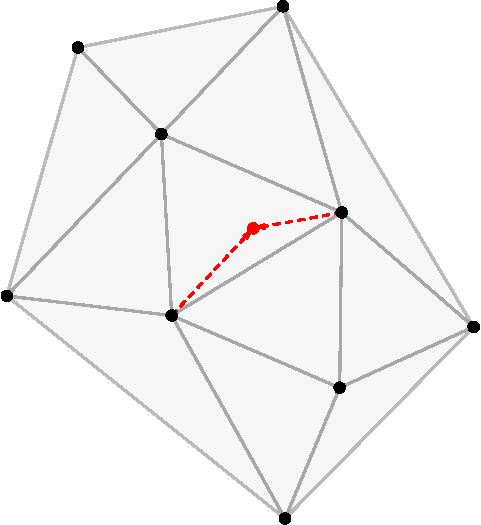
\includegraphics[width=0.45\textwidth]{Figures/schlenker/fundamentals/edgeCollapseACropped.pdf}}
\qquad
\subfloat[Situation nach der Operation]{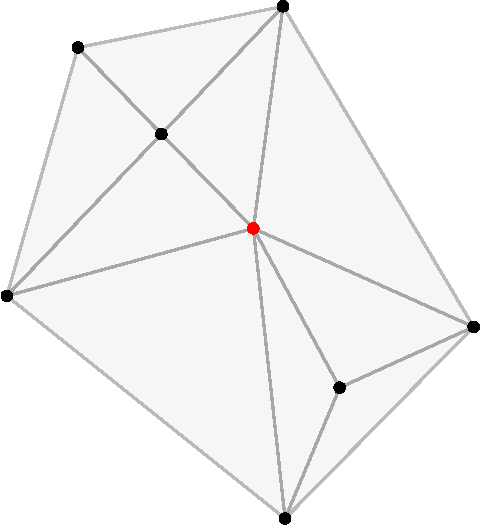
\includegraphics[width=0.45\textwidth]{Figures/schlenker/fundamentals/edgeCollapseBCropped.pdf}}
\caption{Beispiel einer Edge-Collapse-Operation. Die Zielposition der beiden an das Edge angrenzenden Vertices ist \emph{rot} markiert.}
\label{schlenke:fig:fundamentals:edgecollapse}
\end{figure}

Es verbleibt jedoch die Frage, welche Paare von Vertices verschmolzen werden sollen. Hierfür wird in \cite{garland1997} ein Verfahren vorstellt, das mithilfe von Quadriken jeder möglichen Edge-Collapse-Operation einen Wert für die damit verbundenen Kosten zuweist. Iterativ werden nun die Vertices aus Operationen mit den geringsten Kosten verschmolzen, woraufhin die Kosten der Operationen, die sich auf die umliegenden Vertices beziehen, aktualisiert werden müssen.

Der Algorithmus aus \cite{garland1997} ist jedoch nur auf nicht-texturierte Meshes anwendbar. Möchte man dieses Verfahren verwenden, um 3D"=Modelle mit Textur zu komprimieren, so müssen einerseits die Verschmelzungsoperationen auch auf die Texturkoordinaten angewandt werden, was insbesondere entlang von Texture Seams eine sehr sorgfältige Implementierung erfordert, andererseits müssen aber auch diese Texturkoordinaten in die Berechnung der Kosten für die jeweilige Operation miteinbezogen werden. Abweichungen in der resultierenden Oberfläche des 3D"=Modells haben hier Verzerrungen in der Textur zur Folge. Dies gilt auch für Texture Seams, bei welchen es darüber hinaus nicht vermeiden lässt, dass auch Bereiche der als Textur verwendeten Bilddatei für die Einfärbung der Faces verwendet werden, die im ursprünglichen Modell überhaupt nicht parametrisiert waren und somit beliebigen Inhalt aufweisen können. Es empfiehlt sich daher, die Ränder der Bereiche in der Bilddatei mit einem ähnlichen Farbton wie die eigentliche Textur zu färben, was bei den meisten Textur erzeugenden Programmen automatisch geschieht. Die daher notwendige Erweiterung des bestehenden Kompressions-Algorithmus auf texturierte Meshes wird in \cite{garland1998} vorgenommen, wobei Texture Seams dort kaum behandelt werden. Die für die Kompressions-Komponente erstellte Implementierung behandelt jedoch auch diese Bereiche auf eine sinnvolle Art und Weise.

\subsubsection{Kompression der Textur}

Während die Kompression der Modellgeometrie insbesondere bei texturierten Meshes nichttrivial ist, gestaltet sich die Kompression der Texturdaten relativ einfach. Die Textur wird in einer herkömmlichen Bilddatei gespeichert, deren Dateigröße direkt von der Auflösung des darin gespeicherten Bildes abhängt. Wird die Auflösung des Bildes verringert, was der Funktionsumfang eines jeden brauchbaren Bildbearbeitungsprogramms zulässt, schlägt sich dies auch in der Größe der Texturdatei nieder. Darüber hinaus sind weitere aus der Bildverarbeitung bekannte Kompressionsverfahren einsetzbar, wie zum Beispiel die JPEG-Komprimierung\footnote{https://www.ece.ucdavis.edu/cerl/reliablejpeg/compression/}.

Allerdings muss darauf geachtet werden, dass die zusammen mit der Modellgeometrie gespeicherten Texturkoordinaten auch nach der Kompression der Textur wohldefiniert sind. Besonders angenehm ist hier jedoch die Tatsache, dass diese Texturkoordinaten sich nicht auf die Pixel beziehen, sondern stets im Interval von null bis eins liegen, wobei sich null auf den oberen bzw. linken Rand und eins auf den unteren bzgl. rechten Rand der Texturdatei bezieht. Aus diesem Grund sind die Texturkoordinaten gänzlich unabhängig von der Auflösung der die Textur beinhaltenden Bilddatei und diese Datei kann ohne Modifizierung der Geometriedatei komprimiert werden. Diese Aussage gilt nicht nur für die Anpassung der Auflösung, sondern auch für andere Kompressionsverfahren aus der Bildverarbeitung.

\subsection{Voraussetzungen}

Die Kompressions-Komponente dient zur Kompression von Mediendaten, die im Dateimanagement auf dem Lokalen Anwendungsserver (LAS) registriert sind. Die Kompressions"=Komponente läuft innerhalb eines separaten Docker"=Containers auf dem Server, wofür die Software Docker\footnote{\url{https://www.docker.com/}} auf dem als Host"=System fungierenden Server installiert sein muss. Eine direkte Interaktion des Benutzers mit der Kompressions"=Komponente findet in der Regel nicht statt. Es wird jedoch eine Web"=Oberfläche zur Administration und Konfiguration des Systems bereitgestellt. 

Da die zu komprimierenden Dateien auf dem Host"=System gespeichert sind, worauf sowohl von der Medien"=Datenbank als auch von der Kompressions"=Komponente zugegriffen wird, ist es nicht möglich, das Kompressions"=System unabhängig von der Medien"=Datenbank auszuführen. Andernfalls würden in der Medien"=Datenbank hochgeladene Dateien der Kompressions"=Komponente nicht zur Verfügung stehen. 

\subsubsection{Hardwarevoraussetzungen}
\label{schlenke:chp:info:hardware}

Die Anforderungen an die Ressourcen, die sich für den LAS bzw. den Docker"=Container der Kompressions"=Komponente ergeben, hängen in erster Linie von der Größe der zu komprimierenden Mediendateien ab. Während die Prozessorleistung primär die Dauer der Kompressions"=Prozesse bedingt, beschränkt der zur Verfügung stehende Arbeitsspeicher die maximale Größe der Eingabedaten nach oben.
Da der Algorithmus zur Kompression von 3D-Modellen kaum Parallelisierungs"=Möglichkeiten bietet, werden die Berechnungen derzeit nicht auf mehrere Prozessorkerne oder auf die Grafikkarte verlagert. 
Experimente während der Implementierung haben gezeigt, dass Modelle mit ca. 8 Mio. Dreiecken auf einem aktuellen gut ausgestatteten Bürorechner (Intel-Core-i7-Prozessor, 32 GB RAM) komprimiert werden können. Da insbesondere der Arbeitsspeicher der limitierende Faktor ist, spielt jedoch der Speicherbedarf der anderen auf dem System laufenden Anwendungen eine wichtige Rolle.

\subsubsection{Softwarevoraussetzungen}

Die Kompressions-Komponente wurde in der Programmiersprache Java implementiert, weshalb zur Ausführung ein Java Runtime Environment (JRE) im Docker-Container installiert sein muss. Für die Kompression von Bild- und Texturdateien wird im Hintergrund die Software ImageMagick verwendet. Es ergeben sich also die folgenden beiden Software-Abhängigkeiten:
\begin{itemize}
\item Java Runtime Environment\footnote{\url{https://java.com/de/download/}} (getestet mit Version 1.8.0)
\item ImageMagick\footnote{\url{https://imagemagick.org/index.php}} (getestet mit Version 7.0.8)
\end{itemize}
Da diese Software"=Produkte jedoch bei der Installtion des entsprechenden Docker"=Containers automatisch installiert werden, muss dies nicht manuell durch den Benutzer vollzogen werden. 

\subsubsection{Abgrenzungskriterien}

Das Absetzen eines Kompressions-Auftrags wird in der Regel von der Medien"=Datenbank"=Komponente angestoßen. Dennoch wird eine Benutzeroberfläche zum manuellen Absetzen von Kompressions"=Aufträgen zur Verfügung gestellt, die jedoch aufgrund der Notwendigkeit der manuellen Angabe von Identifikatoren keinen hohen Bedienkomfort bietet.

An Medientypen werden Bilder und 3D-Modelle unterstützt. Andere Medientypen können mit dieser Komponente nicht komprimiert werden. An Bilddaten können alle Bildformate komprimiert werden, die von der Software ImageMagick unterstützt werden. An 3D"=Modellen können texturierte und nicht-texturierte Modelle komprimiert werden, die im OBJ"=Format\footnote{\url{http://www.martinreddy.net/gfx/3d/OBJ.spec}} gespeichert werden. Andere Dateien müssen zunächst manuell durch Drittsoftware in das OBJ-Format übersetzt werden. Pro Modell ist aufgrund von Limitierungen in der Medien"=Datenbank maximal eine Material- und eine Texturdatei zulässig. Genauere Informationen über die für ein 3D"=Modell notwendigen und möglichen Dateien sind in folgender \autoref{schlenke:tbl:3d-files} dargestellt. Der implementierte Algorithmus wäre jedoch prinzipiell in der Lage, auch Objekte mit mehreren Texturdateien zu komprimieren.

\begin{table}
\begin{center}
{\footnotesize
\begin{tabular}{llll}
Dateiendung & Informationen & Optional & Notwendigkeit \\
\hline
.obj & Geometriedaten & Nein & Genau eine Datei erforderlich \\
.mtl & Materialdefinitionen & Ja & Maximal eine Datei möglich \\
.jpg/.jpeg/.png & Texturdaten & Ja & Maximal eine Datei, nur falls auch \\
& & & MTL-Datei spezifiziert wird \\
\end{tabular}}
\caption{Für ein 3D"=Modell notwendige und optionale Dateien}
\label{schlenke:tbl:3d-files}
\end{center}
\end{table}

Die in Abschnitt \ref{schlenke:chp:info:hardware} benannten Hardware"=Voraussetzungen gilt es zu beachten.

Bei 3D-Modellen wird vorausgesetzt, dass die Eingabedaten den Voraussetzungen mannigfaltigen Meshes, wie sie in Abschnitt \ref{schlenke:chp:fundamentalsGeometry} beschrieben wurden, genügen. Für Modelle, welche diese Eigenschaft nicht aufweisen, wird keine Garantie bezüglich des Ergebnisses des Kompressionsvorgangs gegeben. Mögliche Konsequenzen sind ein Fehlschlagen des Kompressionsvorgangs oder unbrauchbare Resultate, auch wenn ein Fehlschlagen in den Experimenten nicht beobachtet wurde. Das Eingabemodell sollte möglichst ausschließlich aus Dreiecken bestehen. Faces höherer Ordnung werden beim Einlesen naiv in Dreiecke umgewandelt, wobei auch hier keine Garantie bezüglich der Qualität des Ergebnisses gegeben werden kann. 

Eine Darstellung der Eingangsdaten oder deren komprimierter Versionen findet innerhalb der Kompressions"=Komponente nicht statt. Die Resultate des Kompressionsvorgangs werden lediglich als Datei im System abgelegt.

Die Kompressions"=Komponente bietet keinerlei Benutzerauthentifizierung oder sonstige Zugriffsbeschränkungen. Die Komponente muss anderweitig vor dem Zugriff Dritter geschützt werden. Für den Zugriff auf die API und die Konfigurations- und Administrationsoberfläche kann lediglich eine Whitelist mit IP"=Adressen hinterlegt werden, für welche der Zugriff exklusiv gewährt wird.

\subsection{Funktionsweise}
\label{schlenke:chp:funktionsweise}

Die Kompressions"=Komponente dient zum Abarbeiten von Kompressions"=Aufträgen, wobei letztere die Kompression \emph{einer} medialen Repräsentation eines Objekts in \emph{mehreren} Auflösungsstufen umfasst. Die Medien"=Dateien stehen dem Kompressions"=System über das Dateisystem zur Verfügung. In der Regel wird ein Kompressions"=Auftrag direkt nach dem Hochladen einer Medien"=Datei in die ViSIT"=Medien"=Datenbank abgesetzt.

Bei der Abarbeitung eines Kompressions"=Auftrags werden zunächst die technischen Metadaten aus der Meta"=Datenbank abgerufen. Diese technischen Metadaten werden für jede mediale Repräsentation gespeichert und umfassen wichtige Informationen über die dazugehörigen Medien"=Dateien und die bestehenden Kompressionsstufen. Sie können außerdem Kontext"=Informationen über eine mediale Repräsentation beinhalten, so speichert beispielsweise die Kompressions"=Komponente bei 3D"=Modellen die Anzahl der Vertices und der Faces. Die technischen Metadaten liegen in der Meta"=Datenbank im JSON-Format\footnote{\url{http://www.ecma-international.org/publications/files/ECMA-ST/ECMA-404.pdf}} vor, wobei hierfür die in Listing \ref{schlenke:lst:technicalMetaSpec} dargestellte Spezifikation gilt. Im Anschluss wird unterschieden, ob es sich bei der zu komprimierenden Medien"=Datei um ein Bild oder ein 3D"=Modell handelt. Ausschlaggebend hierfür ist der im Kompressions"=Auftrag angegebene MIME"=Typ.

\begin{lstlisting}[float, caption={Spezifikation des die technischen Metadaten beinhaltenden JSON-Objekts},label=schlenke:lst:technicalMetaSpec]
{
		"title"	: string,
		"description" : string,
		"objectTripleID" : string,
		"objectTripleURL" : string,
		"mediaTripleID" : string,
		"mediaTripleURL" : string,
		"MIMEtype" : string
		"createDate" : timestamp,
		"creatorID" : string,
		"creatorName" : string,
		"rightholder" : string,
		"uploader" : string, 
		"files" : {
				"origin" : {
						"uploadDate" : timestamp,
						"accessLevel" : string,
						"license" : string,
						"fileSize" : long,
						"paths" : [string],
						"fileTypeSpecificMeta" : object
				},
				...
		}
}
\end{lstlisting}

Die beiden in diesem Objekt verwendeten URLs bezeichnen die ID des Metadatums, welches durch die mediale Repräsentation beschrieben wird, in der Meta"=Datenbank ({\ttfamily object\-Triple\-URL}) bzw. die ID der digitalen Repräsentation selbst ({\ttfamily media\-Triple\-URL}), wie in Abbildung \autoref{fig:digrep} veranschaulicht wird. Diese beiden Werte haben die Form einer URL und können somit nicht als Dateinamen verwendet werden, wie es in der Medien"=Datenbank geschieht. Jedoch verwenden alle in diesem Kontext auftretenden URLs das gleiche Präfix, wodurch die Eindeutigkeit auch bei einer Beschränkung auf das Suffix gewährleistet bleibt, welches sich als Dateiname eignet. Das Suffix der {\ttfamily object\-Triple\-URL} wird als {\ttfamily object\-Triple\-ID}, das der {\ttfamily media\-Triple\-URL} als {\ttfamily media\-Triple\-ID} bezeichnet. Ein Beispiel hierzu ist in Abbildung \ref{schlenke:fig:IdAndUrlExample} zu sehen.

\begin{figure}
\[\underbrace{\mbox{\ttfamily http://visit.de/metadb/}\underbrace{\mbox{\ttfamily 7dde4f1c-022f-4489-9f13-d568ab3c7905}}_{\mbox{mediaTripleID}}}_{\mbox{mediaTripleURL}}\] 
\caption{Beziehung von mediaTripleID und mediaTripleURL anhand eines Beispiels}
\label{schlenke:fig:IdAndUrlExample}
\end{figure}

Die Dateien werden in der Medien"=Datenbank im Format
\begin{lstlisting}[caption={Schema der Dateinamen in der Medien-Datenbank, das ebenfalls durch das Kompressions-System verwendet wird}]
objectTripleID.mediaTripleID.compressionLevelID.Dateiendung
\end{lstlisting}
abgespeichert, worauf ebenfalls durch das Kompressions"=System zugegriffen wird. Hierbei bezeichnet {\ttfamily compressionLevelID} die Bezeichnung für die jeweilige Kompressions"=Stufe. Für die Originaldatei wird hierbei {\ttfamily origin} verwendet, für 3D"=Modelle die Vertexanzahl und für Bilder der in der Konfiguration festgelegte Titel für die jeweilige Auflösungsstufe.

Im folgenden wird auf die Semantik der einzelnen Werte dieses JSON-Objekts eingegangen:
\begin{itemize}
\item {\ttfamily title}: Ein vom Benutzer festgelegter Titel des Objekts
\item {\ttfamily description}: Eine vom Benutzer festgelegte Beschreibung des Objekts
\item {\ttfamily objectTripleID}: Wie oben beschrieben
\item {\ttfamily objectTripleURL}: Wie oben beschrieben
\item {\ttfamily mediaTripleID}: Wie oben beschrieben
\item {\ttfamily mediaTripleURL}: Wie oben beschrieben
\item {\ttfamily createDate}: Der UNIX-Timestamp, an dem die Datei in die Medien"=Datenbank geladen wurde
\item {\ttfamily creatorID}: Die Syncthing-ID des Netzwerkteilnehmers, von dem die Datei hochgeladen wurde
\item {\ttfamily creatorName}: Der Name des Netzwerkteilnehmers, von dem die Datei hochgeladen wurde
\item {\ttfamily rightholder}: Der Rechteinhaber an der Medien"=Datei
\item {\ttfamily uploader}: Name der Person, welche die Datei in die Medien"=Datenbank geladen hat
\item {\ttfamily MIMEtype}: MIME-Typ der Medien-Datei (z.~B. \glqq{}image/png\grqq{} für ein PNG"=Bild oder \glqq{}text/plain\grqq{} für ein 3D"=Modell)
\item {\ttfamily files}: Ein Objekt, das für jede zur Verfügung stehende Kompressions"=Stufe (inklusive der Originaldatei) weiterführende Informationen bereitstellt. Diese werden als Objekt in einer Eigenschaft gespeichert, deren Titel der Bezeichnung der jeweiligen Kompressions"=Stufe entspricht, also beispielsweise {\ttfamily origin} für die Originaldatei. Dieses Objekt weist das folgende Schema auf:
	\begin{itemize}
	\item {\ttfamily uploadDate}: Der UNIX-Timestamp, an dem diese Kompressions"=Stufe erstellt wurde
	\item {\ttfamily accessLevel}: Zugriffsberechtigung für die Kompressions"=Stufe in der Medien"=Datenbank, kann entweder {\ttfamily public}, {\ttfamily private} oder {\ttfamily visit} sein
	\item {\ttfamily license}: Lizenz, unter der die Mediendatei in dieser Kompressions"=Stufe verfügbar ist
	\item {\ttfamily fileSize}: Größe der Mediendatei in Bytes (bei 3D"=Modellen mit mehreren Dateien die Summe aller Dateien)
	\item {\ttfamily paths}: Array mit den internen Dateinamen aller zu dieser medialen Repräsentation gehöriger Dateien
	\item {\ttfamily fileTypeSpecificMeta}: Weitere unspezifizierte Informationen zu dieser Kompressions"=Stufe
	\end{itemize}
\end{itemize}

\paragraph{Bilddatei}

Zur Kompression von Bildateien wird im Hintergrund die Software ImageMagick verwendet. Für jede der in der Konfiguration festgelegten Auflösungsstufen, die kleiner als die Originalgröße des Bildes ist, wird damit eine verkleinerte Version des Bildes erstellt. Laut den technischen Metadaten bereits existierende Auflösungsstufen werden dabei übersprungen. Die neu erstellten Auflösungsstufen werden nun den technischen Metadaten hinzugefügt und in die Meta"=Datenbank überführt.

\paragraph{3D-Modell}

Ein texturiertes 3D"=Modell besteht in der Regel aus drei Dateien. Die OBJ"=Datei mit den Geometriedaten verweist auf eine MTL"=Datei, welche die Materialeigenschaften der Oberfläche beschreibt und insbesondere auf vorhandene Textur"=Dateien referenziert. Beim Hochladen eines 3D"=Modells in die Medien"=Datenbank werden die Dateien dort automatisch umbenannt. Die Referenzen, die zwischen den Dateien bestehen, werden dabei jedoch nicht angepasst und daher ungültig. Im ersten Schritt der Kompression werden diese Verweise in den Originaldateien repariert, indem sie an die neuen Dateinamen angepasst werden. Auch die zum unkomprimierten Modell gehörenden technischen Metadaten werden angepasst.

Nachdem das unkomprimierte Modell repariert wurde, kann mit der eigentlichen Kompression begonnen werden. Zunächst werden die Geometriedaten (OBJ"=Dateien) und ggf. auch die Material"=Datei komprimiert und abgespeichert, wobei auch hier laut den technischen Metadaten bereits existierende Auflösungsstufen übersprungen werden. Nachdem alle Varianten der Geometriedaten erstellt wurden, erfolgt bei texturierten Modellen die Kompression der Textur separat für jede Auflösungsstufe, erneut unter der Zuhilfenahme der Software ImageMagick. Die zuvor erstellten Material"=Dateien verweisen bereits auf die nun erstellten Bilddateien. Wie bereits bei den Bilddateien werden abschließend die um die neuen Auflösungsstufen erweiterten technischen Metadaten an die Meta"=Datenbank übertragen.

\subsection{Installation und Steuerung }

\subsubsection{Installation}

Zur Installation des Kompressions"=Systems muss zunächst über den Befehl 
\begin{lstlisting}[caption=Befehl zum Erstellen des Docker-Images]
docker build -t "visitapp/compression" https://github.com/ViSIT-Dev/compressioncontainer.git
\end{lstlisting}
ein Docker"=Image erstellt werden. Nun muss ein Verzeichnis gewählt werden, über das von außen auf die das Kompressions"=System betreffende Dateien, wie die Log"=Dateien oder die Konfiguration zugegriffen wird. Hier werde beispielsweise das Verzeichnis {\ttfamily /etc/visit-compression} gewählt. Anschließend kann über den Befehl
\begin{lstlisting}[caption=Befehl zum Erstellen des Docker-Containers]
docker run -d --name compression -p 1613:1613 -v visit-p2p-private:/var/www/Private -v /etc/visit-compression:/root/compression visitapp/compression
\end{lstlisting}
aus dem soeben erstellten Docker"=Image ein ausführbarer Docker"=Container generiert werden, sofern {visit-p2p-private} das Docker"=Volume bezeichnet, in welchem die Medien"=Dateien gespeichert sind. Die einzelnen Bestandteile dieses Befehls werden im folgenden kurz erläutert:
\begin{itemize}
\item {\ttfamily docker run}: Dies ist der Befehl zum Erstellen eines Docker"=Images.
\item {\ttfamily -d}: Der Container soll im Hintergrund ausgeführt werden.
\item {\ttfamily -p 1613:1613}: Der Port 1613 innerhalb des Docker"=Containers soll zum Host"=System durchgeschleift werden. Sollen andere Ports verwendet werden, muss dieser Bestandteil entsprechend angepasst werden.
\item {\ttfamily -v visit-p2p-private:/var/www/Private}: Das beim Einrichten der Medien"=Datenbank erzeugte Docker"=Volume {\ttfamily visit-""p2p-""private}, in dem die Medien"=Dateien gespeichert sind, soll innerhalb des Docker"=Containers unter dem Pfad {\ttfamily /var/www/Private} verfügbar sein.
\item {\ttfamily -v /etc/visit-compression:/root/compression}: Auf dem Host"=System soll unter dem Verzeichnis {\ttfamily /etc/visit"=compression} auf die Dateien zugegriffen werden können, welche sich innerhalb des Docker"=Containers im Verzeichnis {\ttfamily /root/compression} befinden.
\item {\ttfamily visitapp/compression}: Dies ist die gewählte Bezeichnung für das eben erstellte Docker"=Image.
\end{itemize}
Nach dem Erstellen des Docker"=Containers wird dieser automatisch gestartet und kann, wie im folgenden Abschnitt erläutert wird, beendet oder neu gestartet werden. Bei gestartetem Container ist die Web"=Oberfläche in der Standardkonfiguration unter \url{http://localhost:1613} erreichbar, während die API unter \url{http://localhost:1613/api} zur Verfügung steht. Bevor die Kompressions"=Komponente vollständig funktionstüchtig ist, müssen jedoch die Konfigurationsoptionen geeignet angepasst werden, wobei hierfür auf Abschnitt \ref{schlenke:chp:configuration} verwiesen wird.

\subsubsection{Steuerung des Docker-Containers}

Der die Kompressions"=Komponente beinhaltende Docker"=Container kann wie jeder andere Container mit den Befehlen
\begin{lstlisting}[caption={Kommando zum Beenden des Docker-Containers der Kompressions-Komponente},label=schlenke:lst:dockerstop]
docker stop compression
\end{lstlisting}
gestoppt und mit dem Befehl
\begin{lstlisting}[caption={Kommando zum Starten des Docker-Containers der Kompressions-Komponente}]
docker start compression
\end{lstlisting}
wieder gestartet werden. Alle Einstellungen bleiben dabei erhalten. Über das bei der Installation angegebene Verzeichnis (standardmäßig {\ttfamily /etc/visit-compression}) kann auch außerhalb des Containers auf das Kompressions"=System betreffende Dateien zugegriffen werden. So kann durch Editieren der Datei {\ttfamily config.ini} die Konfiguration angepasst werden, wobei für ein Aktivieren der aktualisierten Einstellungen ein Neustart des Docker"=Containers erforderlich ist. Außerdem kann auf die Log"=Datei {compression.log} zugegriffen werden, die insbesondere bei fehlgeschlagenen Kompressions"=Aufträgen oder bei unerwartetem Beenden des Kompressions"=Systems wichtige Informationen über die zugrunde liegende Ursache liefern kann. Da die Ausgabe dieser Informationen zusätzlich über die Standardausgabe erfolgt, besteht eine weitere Möglichkeit des Zugriffs im Ausführen des Kommandos:
\begin{lstlisting}[caption={Kommando zum Anzeigen der Ausgaben des Kompressions-Systems}]
docker logs compression
\end{lstlisting}
Für fortgeschrittene Benutzer, welche Anpassungen direkt im Docker"=Container vornehmen möchten, kann über den Befehl
\begin{lstlisting}[caption={Befehl zum Öffnen einer Kommandozeile im Kompressions-Container}]
docker exec -it compression /bin/bash
\end{lstlisting}
eine Kommandozeile geöffnet werden.

\subsubsection{Steuerung der Kompressions-Komponente}
\label{schlenke:chp:componentcontrol}

Sämtliche Kommunikation mit der Kompressions"=Komponente selbst erfolgt über die bereitgestellte API. Die zur Verfügung stehende Web"=Oberfläche greift ebenfalls über diese API auf das System zu. Für Details zur Web"=Oberfläche und zur API wird auf die Abschnitte \ref{schlenke:chp:webui} und \ref{schlenke:chp:api} verwiesen.

Die Kompressions"=Komponente startet automatisch nach dem Start des entsprechenden Docker"=Containers. Je nach Konfiguration wird daraufhin unmittelbar mit dem Abarbeiten von Kompressions"=Aufträgen begonnen. 

Die Kompressions"=Komponente lässt sich über entsprechende API"=Aufrufe in unterschiedlichen Modi herunterfahren. Diese Modi umfassen
\begin{itemize}
\item das Abarbeiten aller noch ausstehender Aufträge vor dem Beenden,
\item das Abarbeiten nur des sich aktuell in Verarbeitung befindlichen Auftrags und
\item das sofortige Beenden des Systems ohne Rücksichtnahme auf die ausstehenden Kompressions"=Aufträge.
\end{itemize} 
In jedem Fall werden keine weiteren Kompressions"=Aufträge angenommen. Ausstehende Kompressionsaufträge bleiben beim erneuten Starten der Komponente erhalten. Jedoch wird ein etwaiger Auftrag, der sich während des Beendens in der Verarbeitung befand, als \glqq{}Fehlerhaft abgeschlossen\grqq{} markiert.

Diese Methode des Herunterfahrens erlaubt im Gegensatz zum Stoppen des Docker"=Containers die kontrollierte Handhabung noch ausstehender oder sich in Verarbeitung befindlicher Kompressions"=Aufträge. Allerdings wird durch das Herunterfahren der Kompressions"=Komponente der sie enthaltende Docker"=Container nicht automatisch mit beendet. Dies muss separat durch das Kommando in \autoref{schlenke:lst:dockerstop} erfolgen. Wird der Container mit diesem Kommando ohne vorheriges Herunterfahren des Kompressions"=Systems ausgeführt, entspricht dies dem sofortigen Beenden des Systems ohne Rücksichtnahme auf die ausstehenden Kompressions"=Aufträge.

\subsection{Konfiguration}
\label{schlenke:chp:configuration}

Beim Starten des Kompressions-Systems wird automatisch eine Konfigurationsdatei mit den Standardwerten  unter dem Pfad
\begin{lstlisting}
/root/compression/config.ini
\end{lstlisting} 
angelegt, sofern eine solche nicht bereits an dieser Position existiert. Einige der Werte lassen sich nur manuell über diese Datei anpassen. Auf die wichtigsten Konfigurationsmöglichkeiten kann jedoch auch von außen über die API und die Web-Oberfläche sowohl lesend als auch schreibend zugegriffen werden. Beim manuellen Anpassen der Konfigurationsdatei muss darauf geachtet werden, dass innerhalb der Variablenwerte die Zeichen \glqq{}:\grqq{}, \glqq{}=\grqq{} und \glqq{}\textbackslash\grqq{} mit einem vorgestellten Backslash versehen werden müssen, also beispielsweise durch \glqq{}https\textbackslash ://\grqq{}. Für Details diesbezüglich wird auf die entsprechende Java-Dokumentation\footnote{\url{https://docs.oracle.com/javase/7/docs/api/java/util/Properties.html\# load(java.io.Reader)}} verwiesen. \autoref{schlenke:tbl:configOptions} gibt Aufschluss über alle Konfigurationsmöglichkeiten, welche in den folgenden Abschnitten detailliert erläutert werden.

\begin{table}
\begin{center}
%\resizebox{\textwidth}{!}{
\begin{tabular}{lll}
\hline
Variable & Standard & Web\\
\hline
\multicolumn{3}{c}{Verwaltung von Kompressionsaufträgen} \\
\hline
{\lstinline|accessWhiteListIps|} & {\lstinline|[127.0.0.1,*]|} & {\footnotesize Ja} \\
{\lstinline|apiPort|} & {\lstinline|1613|} & {\footnotesize Ja} \\
{\lstinline|archiveDisplayLength|} & {\lstinline|250|} & {\footnotesize Nein} \\
{\lstinline|autostart|} & {\lstinline|true|} & {\footnotesize Ja} \\
{\lstinline|mediaFileRootDirectory|} & {\lstinline|/var/www/private|} & {\footnotesize Nein} \\
{\lstinline|queueMaxLength|} & {\lstinline|5000|} & {\footnotesize Ja} \\
\hline
\multicolumn{3}{c}{3D-Kompression} \\
\hline
{\lstinline|defaultLevels|} & {\footnotesize siehe Beschreibung} & {\footnotesize Ja} \\
{\lstinline|targetSizeBoundaryPenalty|} & {\lstinline|100.0|} & {\footnotesize Nein} \\
{\lstinline|targetSizeNormalDifferencePenalization|} & {\lstinline|1000.0|} & {\footnotesize Nein} \\
{\lstinline|targetSizeNormalDifferenceThreshold|} & {\lstinline|0.5|} & {\footnotesize Nein} \\
{\lstinline|targetSizePartitionPenalization|} & {\lstinline|10.0|} & {\footnotesize Nein} \\
{\lstinline|targetSizeQualityThreshold|} & {\lstinline|0.3|} & {\footnotesize Nein} \\
{\lstinline|textureLimits|} & {\lstinline|[5000, 50000]|} & {\footnotesize Ja} \\
{\lstinline|textureSizes|} & {\lstinline|[1024, 2048, 8192]|} & {\footnotesize Ja} \\
\hline
\multicolumn{3}{c}{Bildkompression} \\
\hline
{\lstinline|imageCompressionLevels|} & {\footnotesize siehe Beschreibung} & {\footnotesize Ja} \\

\hline
\multicolumn{3}{c}{Schnittstelle Meta-Datenbank} \\
\hline
{\lstinline|metadbApiAuthString|} & {\lstinline|Basic XX...XX\=\=|} & {\footnotesize Nein} \\
{\lstinline|metadbApiEndpointFetchUrl|} & {\lstinline|https\://DOMAIN/metadb-rest-api/digrep/media|} & {\footnotesize Nein} \\
{\lstinline|metadbApiEndpointSendUrl|} & {\lstinline|https\://DOMAIN/metadb-rest-api/digrep/media|} & {\footnotesize Nein} \\
{\lstinline|metadbApiMediaUidPrefix|} & {\lstinline|http\://DOMAIN/metadb/|} & {\footnotesize Nein} \\
\end{tabular}%}
\caption{Überblick über alle Konfigurationsmöglichkeiten der Kompressionskomponente und deren Verfügbarkeit über die Web"=Oberfläche}
\label{schlenke:tbl:configOptions}
\end{center}
\end{table}

\subsubsection{Verwaltung von Kompressionsaufträgen}

Zur Verwaltung der eingehenden Kompressionsaufträge und für die dazu notwendigen Einstellungen des Servers stehen die folgenden Konfigurationsmöglichkeiten zur Verfügung:

\paragraph{Zugriffsbeschränkung} Der Wert von {\ttfamily access\-White\-List\-Ips} beschreibt, über welche Rechner auf die API oder die Web-Oberfläche zugegriffen werden kann, indem die IP-Adressen dieser Rechner angegeben werden können. Generell sollte die Absicherung allerdings auf eine andere Art von außen vorgenommen werden. Die IP-Adressen werden in eckigen Klammern und durch Kommata getrennt notiert. Befindet sich ein Asterisk (\glqq{}$\ast$\grqq{}) in dieser Auflistung, wird der Zugriff für alle Rechner authorisiert. Der Standardwert für diese Eigenschaft ist  {\ttfamily [127.0.0.1, *]}, wodurch keine Beschränkung des Zugriffs erfolgt.

\paragraph{Serverport} Der Wert für die Variable {\ttfamily api\-Port} muss einer Ganzzahl im Intervall von 1 bis 65535 entsprechen und legt den Port fest, über welchen sowohl auf die API als auch auf die Web-Oberfläche der Kompressions-Komponente zugegriffen werden kann. Der Standardwert für diese Variable ist {\ttfamily 1613}.

\paragraph{Länge der Archiv-Anzeige} Über den Parameter {\ttfamily archive\-Display\-Leng\-th} lässt sich festlegen, wie viele Einträge in dem über die Web-Oberfläche zugänglichen Archiv der letzten Kompressions-Aufträge angezeigt werden sollen. Auch dieser Wert muss einer positiven Ganzzahl entsprechen und beträgt standardmäßig {\ttfamily 250}.

\paragraph{Automatischer Start} Der Wert der Eigenschaft {\ttfamily autostart} kann entweder {\ttfamily true} oder {\ttfamily false} entsprechen und legt fest, ob direkt nach dem Starten der Kompressions-Komponente mit der Abarbeitung eingehender Kompressions-Aufträge begonnen werden soll, wobei dieser Fall dem Standard entspricht.

\paragraph{Hauptverzeichnis für Medien-Dateien} Die Konfigurationsoption {\ttfamily media\-File\-Root\-Directory} legt fest, in welchem Verzeichnis innerhalb des Docker-Containers der Kompressions-Komponente die zu komprimierenden Mediendateien gespeichert sind. Etwaige Unterverzeichnisse können für jeden Kompressions-Auftrag separat angegeben werden. In ebendiesem Verzeichnis werden die komprimierten Versionen der Dateien nach der Ausführung des Auftrags auch abgelegt. Der Standardort für diese Dateien ist {\ttfamily /var/www/Private}.

\paragraph{Maximale Länge der Auftragsliste} Mithilfe der Option {\ttfamily queueMaxLength} lässt sich eine Beschränkung für die Länge der Liste der unbearbeiteten Kompressions-Aufträge festlegen. Sollte dieser Wert erreicht sein, werden etwaige eingehende Aufträge abgewiesen. Ist der Wert auf {\ttfamily 0} festgelegt, so erfolgt keine Beschränkung der Liste. Der Standardwert beträgt {\ttfamily 5000}.


\subsubsection{3D-Kompression}

Folgende Optionen stehen zur Konfiguration des Kompressions-Algorithmus für 3D-Modelle zur Verfügung:

\paragraph{Standard-Kompressionsstufen} Der Wert für die Option {\ttfamily default\-Levels} legt fest, welche Auflösungsstufen für 3D-Modelle standardmäßig erzeugt werden sollen. Jede Auflösungsstufe wird dabei durch eine Ganzzahl beschrieben, welche die gewünschte Anzahl an Vertices des komprimierten Modells festlegt. Diese Stufen werden durch Kommata voneinander getrennt und insgesamt von eckigen Klammern umrahmt, wie auch durch den in \autoref{schlenke:lst:defaultLevelsDefault} aufgeführten Standardwert 
\begin{lstlisting}[caption={Standardwert für die Konfigurationsoption {\ttfamily default\-Levels}},label=schlenke:lst:defaultLevelsDefault]
	[500, 1000, 5000, 20000, 50000, 200000, 500000, 2000000, 5000000, 20000000, 50000000]
\end{lstlisting}
 deutlich wird. Hat das ursprüngliche Modell bereits weniger Vertices als die angestrebte Anzahl einer Auflösungsstufe, so wird diese Stufe übersprungen anstatt ein Modell mit einer größeren Anzahl an Vertices zu erzeugen.

\paragraph{Bestrafungen von Abweichungen am Rand} Der Gleitkommawert für die Eigenschaft {\ttfamily target\-Size\-Boundary\-Penalty} ist nur für die Kompression von Meshes mit Rand, die also kein vollständiges Modell eines realen Objekts darstellen, relevant. Er legt fest, mit welchem Gewicht dieser Rand des ursprünglichen Modells beibehalten werden soll. Bei einem hohen Wert dieser Eigenschaft werden durch die Kompression kaum Änderungen an diesen Rändern vorgenommen, während bei einem niedrigen Wert viele Edge"=Collapse"=Operationen genau dort ausgeführt werden. Der Standardwert beträgt {\ttfamily 100.0}.

\paragraph{Bestrafungen bei Abweichungen der Oberflächennormale} Die Oberflächennormale ist eine Richtung, welche die Ausrichtung eines Face beschreibt und somit senkrecht zur Ebene, welche durch das Face erzeugt wird, verläuft. Über die beiden Eigenschaften {\ttfamily target\-Size\-Normal\-Difference\-Penalization} und {\ttfamily target\-Size\-Normal\-Difference\-Threshold} lässt sich festlegen, in welchem Ausmaß starke Veränderungen dieser Normalen vermieden werden sollen. Der Wert von {\ttfamily target\-Size\-Normal\-Difference\-Threshold} beschreibt dabei, ab welcher Abweichung der durch eine Edge"=Collapse"=Operation verursachten Veränderung von Oberflächennormalen eine Bestrafung erfolgt, welche die Ausführung dieser Operation unwahrscheinlicher macht, indem die Kosten der Operation mit dem Faktor {\ttfamily target\-Size\-Normal\-Difference\-Penalization} multipliziert werden. Perfekt übereinstimmende Normalen entsprechen dabei dem Wert {\ttfamily 1.0}, während zueinander senkrechte Normalen durch den Wert {\lstinline|0.0|} beschrieben werden. Entsteht durch eine Edge"=Collapse"=Operation ein Face, dessen Oberflächennormale eine Übereinstimmung mit der ursprünglichen Normale hat, die unter dem Wert von {\ttfamily target\-Size\-Normal\-Difference\-Threshold} liegt, so wird dieser Bestrafungsfaktor aktiviert.

\paragraph{Bestrafungen entlang von Texture Seams} Wie in Abschnitt \ref{schlenke:chp:fundamentals:geocomp} erläutert wurde, sorgen Edge"=Collapse"=Operationen entlang von Texture Seams nicht nur zu Verzerrungen in der Textur, sondern können auch die Darstellung von eigentlich nicht parametrisierten Bereichen in der Texturdatei zur Folge haben, was es möglichst zu vermeiden gilt. Aus diesem Grund werden Kompressionsoperationen entlang von Texture Seams mit einem Faktor bestraft, der sich im Wesentlichen aus dem Produkt des Quadrats der an die kollabierende Kante angrenzenden Texturpartitionen und des Werts der Eigenschaft {\ttfamily target\-Size\-Partition\-Penalization} ergibt, wobei letzterer standardmäßig auf {\ttfamily 10.0} festgelegt ist.

\paragraph{Schwellwert für die Begünstigung wohlgeformter Faces} Bei der Erzeugung von Meshes werden in der Regel möglichst gleichmäßige Faces angestrebt, während hingegen sehr lange aber dünne Dreiecke unerwünscht sind. Als Maß für diese \glqq{}Schönheit\grqq{} eines Faces wird der Quotient aus Fläche und maximaler Seitenlänge betrachtet. Die Kosten einer Edge"=Collapse"=Operation werden durch die minimale Qualität der durch diese Operation entstehenden Faces dividiert, wodurch allerdings bei sehr wohlgeformten Faces und demzufolge hoher Qualität die Kosten der gesamten Operation unerwünscht stark sinken können. Aus diesem Grund lässt sich durch den Paramter {\ttfamily target\-Size\-Quality\-Threshold} der Divisor nach oben beschränken, wobei der Standardwert {\ttfamily 0.3} beträgt und somit auch nicht perfekt geformte Dreiecke ohne Erhöhung der Kosten zulässt.

\paragraph{Texturkompression} Durch die Textur eines 3D"=Modells kann ein relevanter Anteil des insgesamt notwendigen Speicherbedarfs verursacht werden, weshalb es auch diesen Bestandteil zu komprimieren gilt. Dies sollte je nach gewählter Vertexanzahl in einem ähnlichen Ausmaß geschehen. Allerdings können viele Programme nur Texturdateien mit einer Zweierpotenz als Seitenlänge verarbeiten oder erweitern die gegebene Textur durch Padding zu einer solchen Größe. Aus diesem Grund ist eine pixelgenaue Wahl der Texturauflösung nur bedingt sinnvoll. Stattdessen kann einem bestimmten Intervall an Vertexanzahlen eine bestimmte Texturauflösung zugewiesen werden. Dies lässt sich über die beiden Parameter {\ttfamily texture\-Limits} und {\ttfamily textur\-Sizes} konfigurieren, wobei beide Parameter Listen mit ganzzahligen Einträgen als Werte akzeptieren. Die Einträge in diesen Listen werden wie bereits bei anderen Konfigurationsoptionen durch Kommata getrennt, während die ganze Liste durch eckige Klammern eingefasst wird. Zu beachten ist jedoch, dass die Anzahl an Einträgen in {\ttfamily texture\-Sizes} stets um genau eins größer sein muss, als die Anzahl der Einträge in {\ttfamily texture\-Limits}. 

Hat ein Modell nun weniger Vertices als der erste Eintrag in der Schwellwert-Liste {\ttfamily texture\-Limits}, so wird eine Textur erzeugt, deren Auflösung dem ersten Eintrag in {\ttfamily texture\-Sizes} entspricht. Hat es stattdessen mindestens so viele Vertices wie der erste Eintrag in {\ttfamily texture\-Limits}, jedoch weniger Vertices als der zweite Eintrag in {\ttfamily texture\-Limits} vorgibt, so wird eine Textur mit einer Seitenlänge entsprechend des zweiten Eintrags in {\ttfamily texture\-Sizes} erzeugt. Diese Regel gilt entsprechend für jeden Eintrag in {\ttfamily texture\-Limits}. Standardmäßig sind die Schwellwerte {\ttfamily texture\-Limits} festgelegt durch {\ttfamily [5000, 50000]}, während die dazugehörigen Auflösungen durch {\ttfamily [1024, 2048, 8192]} gegeben sind. Bei Bedarf lässt sich diese Konfiguration feiner gestalten und dabei insbesondere auch ein Intervall festlegen, das Texturdateien mit einer Seitenlänge von 4096 Pixeln erzeugt. \autoref{schlenke:tbl:textureResolutionExamples} veranschaulicht die resultierenden Texturauflösungen abhängig von unterschiedlichen Vertexanzahlen für die Standardkonfiguration. 

Ist die Auflösung der ursprünglichen Texturdatei jedoch kleiner als die sich bei der Kompression ergebende Größe, so wird die Textur nicht vergrößert, sondern es wird die Datei in der ursprünglichen Auflösung unverändert übernommen.

\begin{table}
\begin{center}
\begin{tabular}{ll}
Vertexanzahl & Texturauflösung \\
\hline
1000 & 1024 x 1024 \\
5000 & 2048 x 2048 \\
10000 & 2048 x 2048 \\
75000 & 8192 x 8192 \\
\end{tabular}
\caption{Beispiele für die sich bei unterschiedlichen Vertexanzahlen ergebenden Texturauflösungen bei der Standardkonfiguration.}
\label{schlenke:tbl:textureResolutionExamples}
\end{center}
\end{table}

\subsubsection{Bildkompression}

Ähnlich wie bei den 3D"=Modellen sollen auch bei Bildern unterschiedliche Auflösungen vorgehalten werden, um für verschiedene Anwendungsfälle eine passende Größe zur Verfügung zu haben. Welche Auflösungen bei der Kompression einer Bilddatei erstellt werden sollen, wird durch die Konfigurationsoption {\ttfamily image\-Compression\-Levels} festgelegt. Aufgrund der Komplexität dieses Parameters muss dieser im JSON"=Format\footnote{\url{http://www.ecma-international.org/publications/files/ECMA-ST/ECMA-404.pdf}} angegeben werden. Der Wert der Konfigurationsoption muss einem Array aus Objekten entsprechen, wobei jedes Objekt die in \autoref{schlenke:tbl:imageCompressionLevelDecl} dargestellten Eigenschaften aufzuweisen hat. Jeder Eintrag des Arrays definiert auf diese Art eine Kompressions-Stufe für ein Bild. Ist das Bild in mindestens einer Dimension kleiner als eine bestimmte Kompressionsstufe, so wird die Erzeugung einer Version mit dieser Auflösung komplett übersprungen, es wird also im Gegensatz zur Texturkompression nicht die ursprüngliche Auflösung verwendet. Der Standardwert für diesen Parameter ist in \autoref{schlenke:lst:imageCompressionLevelsDefault} dargestellt.

\begin{table}
\begin{center}
\begin{tabular}{lll}
Name & Wertebereich & Beispiel \\
\hline
maxWidth & Positive Ganzzahl & 1920 \\
maxHeight & Positive Ganzzahl & 1080 \\
title & A bis Z, a bis z, Binde-, Unterstriche & \glqq{}FullHD\grqq{} \\
\end{tabular}
\caption{Pro Kompressionsstufe notwendige Parameter bei der Bildkompression}
\label{schlenke:tbl:imageCompressionLevelDecl}
\end{center}
\end{table}

\begin{lstlisting}[caption={Standardwert für die Konfigurationsoption {\ttfamily image\-Compression\-Levels}},label=schlenke:lst:imageCompressionLevelsDefault]
	[{"maxWidth"\:3840,"maxHeight"\:2160,"title"\:"UHD"}, {"maxWidth"\:1920,"maxHeight"\:1080,"title"\:"FullHD"}, {"maxWidth"\:800,"maxHeight"\:600,"title"\:"Mittel"}, {"maxWidth"\:120,"maxHeight"\:120,"title"\:"Klein"}]
\end{lstlisting}

\subsubsection{Schnittstelle Meta-Datenbank}

Um die während des Kompressionsvorgangs erstellen Modelle im ViSIT"=System zu registrieren, müssen die zu der Mediendatei gehörigen technischen Metadaten, die in Listing \ref{schlenke:lst:technicalMetaSpec} spezifiziert wurden, in der Meta"=Datenbank aktualisiert werden. Hierzu muss auf diese Datenbank zugegriffen werden können, wofür die nachfolgend erläuterten Parameter anzugeben sind. Alle in diesem Abschnitt angegebenen Konfigurations"=Optionen müssen nach der Installation angepasst werden, um die Integration in das Gesamtsystem zu ermöglichen. In sämtlichen Standardwerten ist {\ttfamily DOMAIN} durch die jeweilige Domain, über welche auf die Meta"=Datenbank zugegriffen werden kann, zu ersetzen.

\paragraph{Authorisierung zum Zugriff auf die Metadaten} Um die Meta-Datenbank durch unbefugten Zugriff zu schützen, müssen sich zugelassene Benutzer oder Systeme authentifizieren. Diese Authentifizierung erfolgt durch das \emph{HTTP Basic Authentication}-Verfahren \footnote{\url{https://tools.ietf.org/html/rfc2617}}. Der dafür notwendige Base64-codierte Authentifizierungs-String, dem die Zeichenfolge \glqq{}{\ttfamily Basic }\grqq{} vorausgeht, muss in der Konfigurationsoption {\ttfamily metadb\-Api\-Auth\-String} angegeben werden, welche nach der Installation der Kompressions-Komponente auf einen gültigen Wert zu setzen ist. Der (ungültige) Standardwert ist in \autoref{schlenke:lst:metadbApiAuthStringDefault} dargestellt.

\begin{lstlisting}[caption={Standardwert für die Konfigurationsoption {\ttfamily metadb\-Api\-Auth\-String}},label=schlenke:lst:metadbApiAuthStringDefault]
	Basic XXXXXXXXXXXXXXXXXXXXXXXXXXXXXX\=\=
\end{lstlisting}

\paragraph{Endpunkt zum Abrufen der Metadaten} In der Konfigurationsoption {\ttfamily metadb\-Api\-Endpoint\-Fetch\-Url} kann der Endpunkt der API zur Meta-Datenbank spezifiziert werden, über den technische Metadaten abgerufen werden können. Dieser Wert ist standardmäßig festgelegt auf {\ttfamily https\textbackslash ://DOMAIN/metadb-rest-api/digrep/media}.

\paragraph{Endpunkt zum Schreiben der Metadaten} Mithilfe der Konfigurationsoption {\ttfamily metadb\-Api\-Endpoint\-Send\-Url} kann der Endpunkt der API zur Meta-Datenbank spezifiziert werden, über den technische Metadaten gespeichert werden können. Auch hier wird der Wert {\ttfamily https\textbackslash ://DOMAIN/metadb-rest-api/digrep/media} als Standard verwendet, da er in der Regel mit dem Wert für {\ttfamily metadb\-Api\-Endpoint\-Fetch\-Url} übereinstimmt.

\paragraph{Präfix der Medien-UIDs} Jede in der Meta-Datenbank registrierte mediale Repräsentation wird durch eine eindeutige sogenannte UID identifiziert. Jede UID beginnt mit einem allen Mediendateien gemeinsamen Präfix, auf welches ein für das Objekt spezifischer alphanummerischer Identifikator folgt. Da zum Starten eines Kompressionsvorgangs durch die Medien-Datenbank nur das alphanummerische Suffix übermittelt wird, muss in der Konfigurationsoption {\ttfamily metadb\-Api\-Media\-Uid\-Prefix} das konstante Präfix festgelegt werden. Der Standardwert, der gegeben ist durch {\ttfamily http\textbackslash ://DOMAIN/metadb/}, muss vor dem ersten Start der Kompressionskomponente geeignet angepasst werden.

\subsection{Zugriff über die Web-Oberfläche}
\label{schlenke:chp:webui}

Auf die Web"=Oberfläche kann über jeden Browser zugegriffen werden, indem eine Verbindung mit dem Docker"=Container auf dem in der Konfiguration festgelegten Port aufgebaut wird. Auf dem Server kann beispielsweise in der Standardkonfiguration, und sofern der Port durch die Docker"=Konfiguration nicht umgeleitet wird, durch die Eingabe der in \autoref{schlenke:lst:webAccessUrl} dargestellten Zeichenfolge die Startseite der Kompressions"=Komponente aufgerufen werden.
\begin{lstlisting}[caption={Zugriff auf die Web-Oberfläche der Kompressions-Komponente},label=schlenke:lst:webAccessUrl]
	http://localhost:1613
\end{lstlisting}
Die Web-Oberfläche bietet vier verschiedene Ansichten, welche im Folgenden erläutert werden. Zwischen diesen Ansichten kann über die Navigation in der linken Seitenleiste bzw. über das Aufklapp"=Menü auf der linken Seite gewechselt werden.

\subsubsection{Startseite}

Die Startseite hat zwei wichtige Funktionen. Zum einen erlaubt sie das Pausieren oder Fortführen der Auftragsverarbeitung und das Herunterfahren des Systems in den in Abschnitt \ref{schlenke:chp:componentcontrol} beschriebenen Modi, zum anderen gibt sie einen Überblick über die aktuell ausstehenden Kompressions-Aufträge, die sich dort auch abbrechen lassen. Wie in \autoref{schlenke:fig:webuiOverview} deutlich wird, werden zu jedem ausstehenden Auftrag mehrere Informationen angezeigt. Diese umfassen neben dem aktuellen Status des Auftrags den Titel, UID und Dateityp des Objekts, die gewünschten Kompressionsstufen, sowie die Zeitpunkte der Absetzung des Auftrags und der letzten Statusänderung. Über die rote Schaltfläche im rechten oberen Bereich eines Auftrags wird dieser nach dem Bestätigen einer Sicherheitsabfrage abgebrochen, sofern sich dieser noch nicht in Verarbeitung befindet. Kompressionsaufträge, die bereits ausgeführt werden, lassen sich nicht abbrechen. Die Auflistung der ausstehenden Kompressionsaufträge erfolgt aufsteigend nach dem Zeitpunkt der Absetzung.

\begin{figure}
\begin{center}
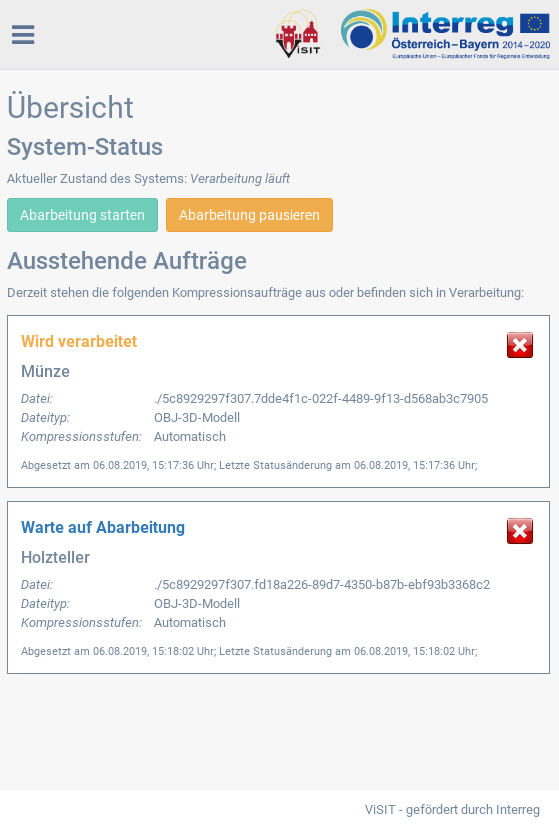
\includegraphics[width=0.55\textwidth]{Figures/schlenker/webui/overview.png}
\caption{Startseite, unter anderem mit einem Überblick über die laufenden und anstehenden Kompressions-Aufträge}
\label{schlenke:fig:webuiOverview}
\end{center}
\end{figure}

\subsubsection{Neuer Auftrag}

Über diese Seite, welche in \autoref{schlenke:fig:webuiDispatch} dargestellt ist, lassen sich manuelle Kompressionsaufträge absetzen, wobei dies normalerweise direkt beim Hochladen der Medien"=Datei von der Medien"=Datenbank übernommen wird. Soll dennoch manuell ein Auftrag abgesetzt werden, so müssen in dieser Ansicht die UID des Metadatums (Objekt-Identifikator, {\ttfamily objectID}) und die UID der digitalen Repräsentation (Medien-Identifikator, {\ttfamily mediaID}), deren Beziehung in Abbildung \autoref{fig:digrep} veranschaulicht wird, angegeben werden. Zusätzlich kann ein Unterverzeichnis angegeben werden (Basis-Pfad), in dem sich die zu komprimierende Datei befindet, wobei dieser Pfad stets in Bezug auf das in der Konfiguration angegebene {\ttfamily media\-File\-Root\-Directory} interpretiert wird. Außerdem muss ein Titel für die Datei angegeben werden, der beliebig gewählt werden kann und lediglich zur leichteren Identifizierung des Auftrags innerhalb des Kompressions-Systems dient. Des weiteren ist der Dateityp zu spezifizieren, wobei hier die Optionen PNG"=Bild, JPEG"=Bild und OBJ"=3D"=Modell zur Auswahl stehen. 

Für den Fall, dass ein 3D"=Modell komprimiert wird, können im darauffolgenden Abschnitt die gewünschten Kompressionsstufen festgelegt werden. Zum Einen steht die Option \glqq{}Automatisch\grqq{} zur Verfügung, die standardmäßig ausgewählt ist und alle in der Konfiguration spezifizierten Standard"=Kompressionsstufen umfasst. Weitere oder alternative Auflösungsstufen können durch die Wahl des Eintrags \glqq{}Feste Größe\grqq{} und die Angabe der gewünschten Vertex"=Anzahl hinzugefügt werden. Sämtliche derzeit angegebenen Auflösungsstufen werden aufgelistet und lassen sich mit Klick auf das Mülltonnen"=Symbol wieder entfernen.

\begin{figure}
\begin{center}
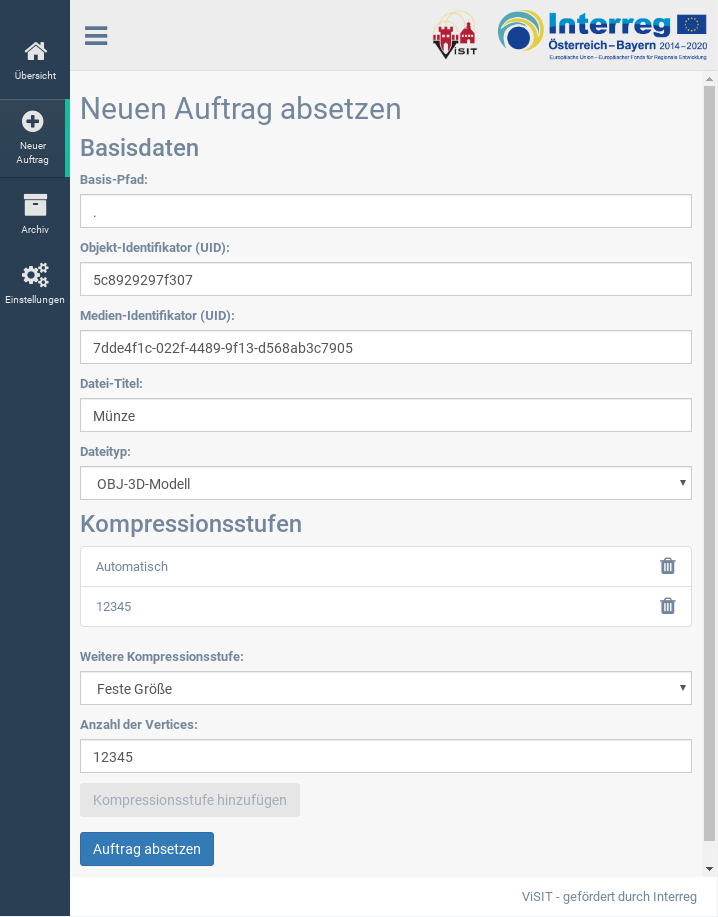
\includegraphics[width=0.55\textwidth]{Figures/schlenker/webui/dispatch2.png}
\caption{Ansicht zum Absetzen eines neuen Kompressions-Auftrags}
\label{schlenke:fig:webuiDispatch}
\end{center}
\end{figure}

\subsubsection{Archiv}

Über diese Ansicht lässt sich ein Überblick über die zuletzt abgearbeiteten Kompressions"=Aufträge erhalten, unabhängig davon, ob die Ausführung erfolgreich war oder fehlgeschlagen ist. Die Einträge werden nach der letzten Statusänderung absteigend sortiert, wobei die Anzahl der dargestellten Einträge in der Konfiguration festgelegt werden kann. Ein Beispiel für diese Ansicht ist in \autoref{schlenke:fig:webuiArchive} zu sehen.

\begin{figure}
\begin{center}
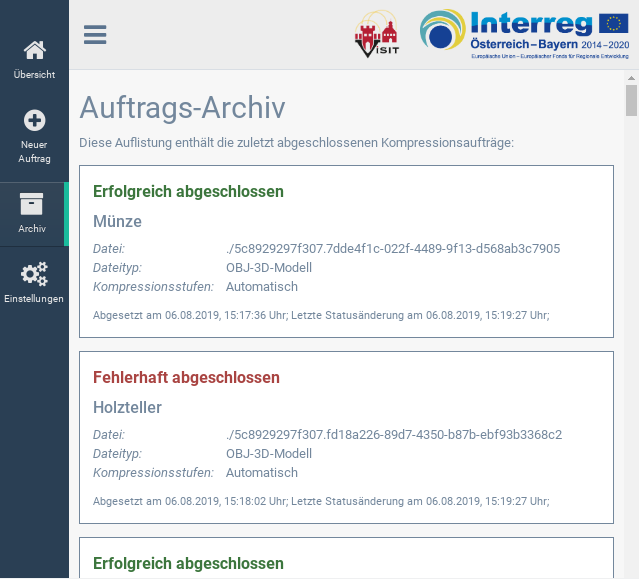
\includegraphics[width=0.55\textwidth]{Figures/schlenker/webui/archive.png}
\caption{Archiv-Ansicht mit einem Überblick über die ausgeführten Kompressions-Aufträge}
\label{schlenke:fig:webuiArchive}
\end{center}
\end{figure}

\subsubsection{Einstellungen}

Auf dieser Seite lassen sich die wichtigsten Konfigurations"=Optionen anpassen, wie in \autoref{schlenke:fig:webuiConfig} zu sehen ist. Alle Einstellungen, die auf dieser Seite nicht verfügbar sind, müssen manuell in der Konfigurationsdatei angepasst werden. Für Details zu den einzelnen Optionen wird auf Abschnitt \ref{schlenke:chp:configuration} verwiesen.

Die über die Web"=Oberfläche verfügbaren Konfigurationsmöglichkeiten werden im Folgenden aufgeführt, wobei auch die Entsprechung in der Konfigurationsdatei benannt wird. Sämtliche Angaben werden jedoch erst durch das Betätigen der Schaltfläche \glqq{}Einstellungen speichern\grqq{} am Ende der Seite zum Server übertragen und übernommen.
\begin{itemize}
\item \emph{Portnummer der API-Schnittstelle: } {\ttfamily apiPort}
\item \emph{Maximale Länge der Auftragsliste: } {\ttfamily queueMaxLength}
\item \emph{Abarbeitung automatisch beim Starten des Servers beginnen: } {\ttfamily autostart}
\item \emph{API"=Zugriffsberechtigte IP-Adressen: }{\ttfamily access\-White\-List\-Ips}. Die berechtigten IP-Adressen sind einzeln anzugeben und über die Schaltfläche \glqq{}IP-Adresse hinzufügen\grqq{} zu bestätigen. Durch einen Klick auf das Mülltonnen"=Symbol können Einträge wieder entfernt werden. Auch hier entspricht die Angabe eines Asterisks (\glqq{}$\ast$\grqq{}) einer Zugriffsgenehmigung für alle Hosts.
\item \emph{Standard-Kompressionsstufen für 3D-Modelle: }{\ttfamily defaultLevels}. Die Anzahl der Vertices der komprimierten Modelle, die bei der Kompression von 3D"=Modellen standardmäßig erstellt werden sollen, sind an dieser Stelle einzeln anzugeben und über die Schaltfläche \glqq{}Kompressionsstufe hinzufügen\grqq{} hinzuzufügen. Auch hier können einzelne Kompressionsstufen durch Betätigen des Mülleimer"=Symbols entfernt werden.
\item \emph{Kompression der Textur von 3D-Modellen: }{\ttfamily textureLimits}, {\ttfamily textureSizes}. Die Anzahl der Schwellwerte und demzufolge unterschiedlicher Textur-Auflösungen lässt sich über die beiden Schaltflächen \glqq{}Unterscheidung hinzufügen\grqq{} bzw. \glqq{}Unterscheidung entfernen\grqq{} kontrollieren. Die Texturgröße ist als Anzahl der Pixel pro Dimension zu verstehen.
\item \emph{Aktionen für die Kompression von Bildern: }{\ttfamily imageCompressionLevels}. Die für eingehende Bild"=Kompressions"=Aufträge zu erstellenden Auflösungsstufen sind hier aufgelistet, wobei sich einzelne Einträge durch das Betätigen des Mülleimer"=Symbols entfernen lassen. Weitere Kompressionsstufen lassen sich durch die Angabe eines beliebigen Titels, der nur aus Groß- oder Kleinbuchstaben, Ziffern und Binde- oder Unterstrichen bestehen darf, sowie der maximalen Breite und maximalen Höhe des komprimierten Bildes in Pixeln und anschließendes Betätigen der Schaltfläche \glqq{}Kompressionsstufe hinzufügen\grqq{} hinzufügen.
\end{itemize}

\begin{figure}
\centering
\subfloat{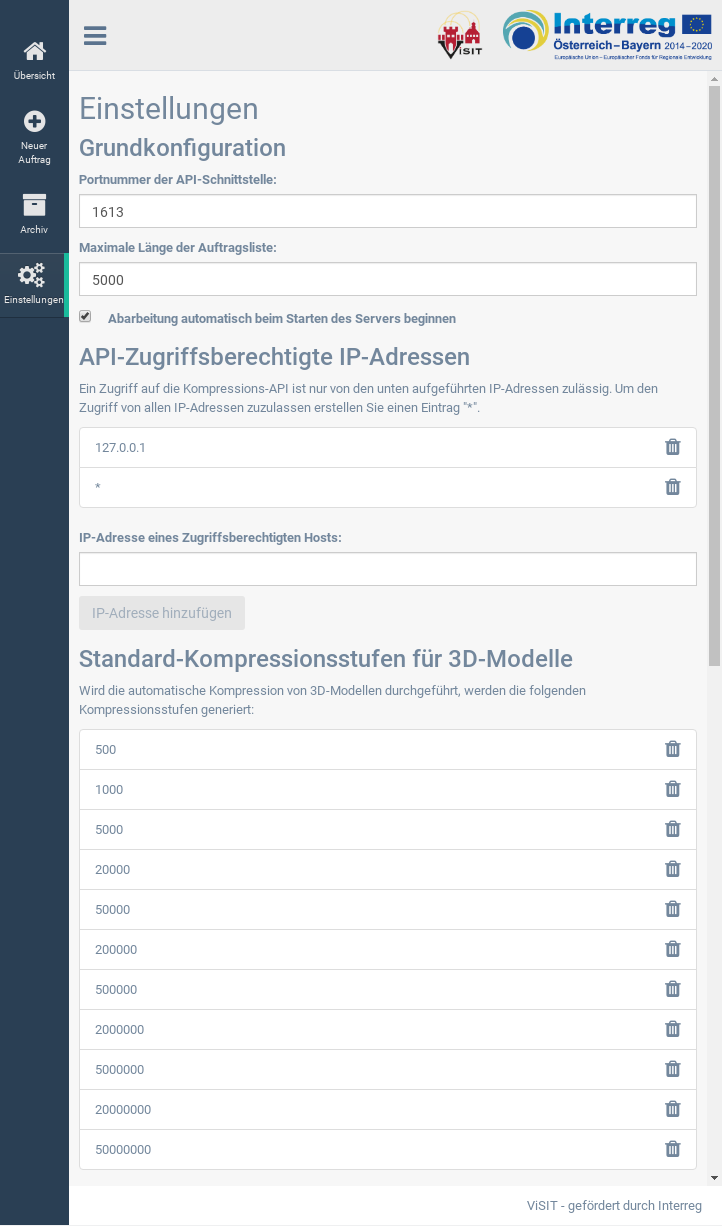
\includegraphics[width=0.45\textwidth]{Figures/schlenker/webui/config1.png}}
\qquad
\subfloat{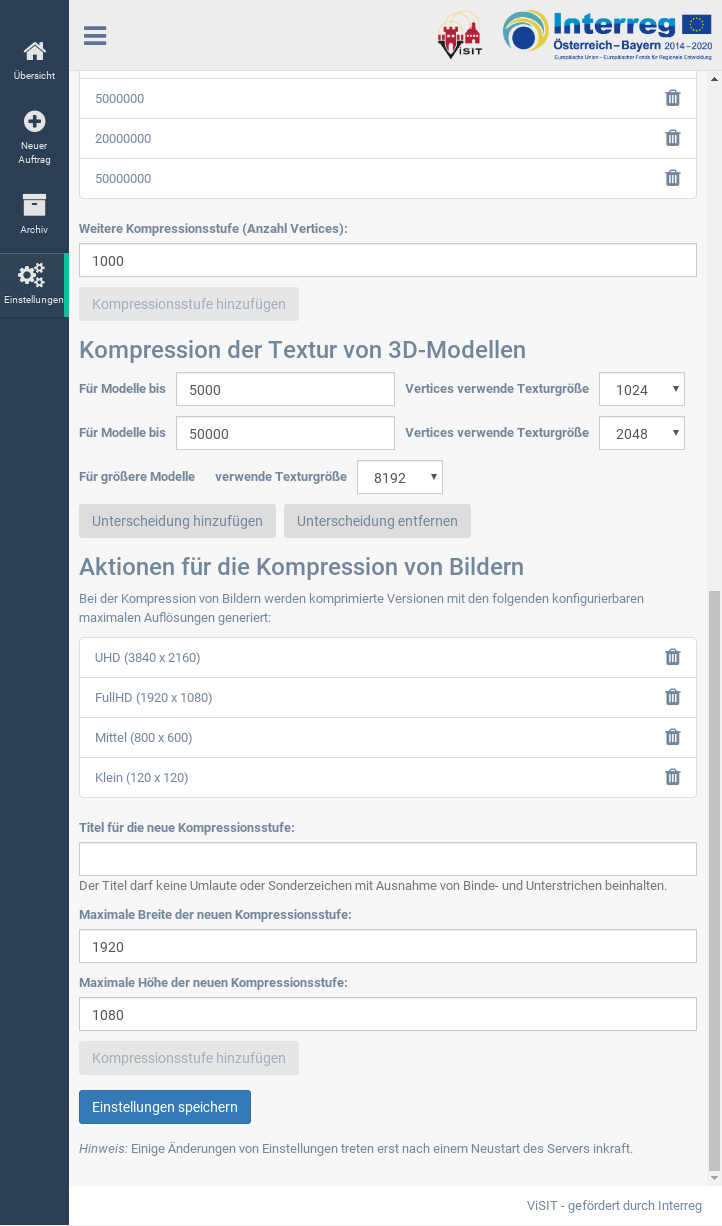
\includegraphics[width=0.45\textwidth]{Figures/schlenker/webui/config2.png}}
\caption{Einstellungsmöglichkeiten über die Web-Oberfläche}
\label{schlenke:fig:webuiConfig}
\end{figure}

\subsection{Zugriff über die API}
\label{schlenke:chp:api}

Sämtliche Funktionen der API stehen bei der standardmäßigen Konfiguration unter dem Basispfad \url{http://localhost:1613/api} zur Verfügung. Die API bietet unterschiedliche Module an, auf deren Funktionen in diesem Abschnitt eingegangen wird. POST"=Parameter sind stets als JSON"=Objekt zu übergeben, ebenso erfolgt die Antwort in Form eines JSON"=Objekts. 

\subsubsection{Aktuelle Kompressions-Aufträge}

Für Informationen zu den IDs, dem MIME"=Typen oder den Kompressions"=Stufen wird auf Abschnitt \ref{schlenke:chp:funktionsweise} verwiesen. Beim Absetzen wird jedem Kompressions"=Auftrag eine ID zugewiesen, welche zum Löschen des Auftrags angegeben werden muss. Der Status eines Auftrags kann einen der folgenden Werte annehmen:
\begin{itemize}
\item {\ttfamily ENQUEUED}: Der Auftrag wurde abgesetzt, mit der Abarbeitung wurde jedoch noch nicht begonnen.
\item {\ttfamily PROCESSING}: Der Auftrag wurde abgesetzt und befindet sich derzeit in Verarbeitung.
\item {\ttfamily ERROR}: Die Verarbeitung des Auftrags wurde fehlerhaft abgeschlossen.
\item {\ttfamily COMPLETED}: Die Verarbeitung des Auftrags wurde erfolgreich abgeschlossen.
\end{itemize}

\noindent\textbf{Funktion: }Absetzen eines Kompressions-Auftrags\\
\textbf{HTTP-Methode: } {\ttfamily POST} \\
\textbf{Pfad: } {\ttfamily /jobs/dispatch} \\
\textbf{POST-Paramter: }
\begin{lstlisting}[caption={POST-Parameter zum Absetzen eines Kompressions-Auftrags}]
{
		basePath : string, 	/* Unterverzeichnis, in welchem die Datei abgelegt ist, ansonsten "" */
		objectUid : string, /* objectTripleID (nicht objectTripleURL) der Medien-Datei */
		mediaUid : string, 	/* mediaTripleID (nicht mediaTripleURL) der zu komprimierenden Medien-Datei */
		title : string, 	  /* Beliebiger Titel zur Identifizierung des Kompressions-Auftrags */
		mimeType : string, 	/* MIME-Typ der zu komprimierenden Datei */
		levels : [string], 	/* Array mit den Bezeichnern aller gewuenschten Kompressions-Stufen */
}
\end{lstlisting}
\textbf{Antwort: }
\begin{lstlisting}[caption={Antwort auf das Absetzen eines Kompressions-Auftrags}]
{
		success : boolean,
		message : string
}
\end{lstlisting}

\noindent\textbf{Funktion: }Auflisten aller noch nicht abgeschlossenen Kompressions-Aufträge\\
\textbf{HTTP-Methode: } {\ttfamily GET} \\
\textbf{Pfad: } {\ttfamily /jobs/dispatch} \\
\textbf{Antwort: }
\begin{lstlisting}[caption={Antwort auf das Auflisten nicht abgeschlossener Kompressions-Aufträge}]
{
		success : boolean,
		message : string,
		items : [{
				job : {
						basePath : string, 	/* Unterverzeichnis, in welchem die Datei abgelegt ist, ansonsten "" */
						objectUid : string, /* objectTripleID (nicht objectTripleURL) der Medien-Datei */
						mediaUid : string, 	/* mediaTripleID (nicht mediaTripleURL) der Medien-Datei */
						title : string, 	  /* Beliebiger Titel zur Identifizierung des Kompressions-Auftrags */
						mimeType : string, 	/* MIME-Typ der zu komprimierenden Datei */
						levels : [string], 	/* Array mit den Bezeichnern aller gewuenschten Kompressions-Stufen */
				},
				receivedOn : timestamp,     /* UNIX-Timestamp, an dem der Auftrag abgesetzt wurde */
				id : int,                   /* Vom Kompressions-System vergebene ID fuer den Auftrag */
				state : string,             /* Aktueller Status des Auftrags, kann entweder ENQUEUED, PROCESSING, ERROR oder COMPLETED sein */
				lastStateChange : timestamp /* UNIX-Timestamp der letzten Statusaenderung des Auftrags */
		}]
}
\end{lstlisting}

\noindent\textbf{Funktion: }Löschen eines Kompressions-Auftrags\\
\textbf{HTTP-Methode: } {\ttfamily DELETE} \\
\textbf{Pfad: } {\ttfamily /jobs/cancel/\{ID\}}, mit \{ID\} der ID des Kompressions"=Auftrags \\
\textbf{Antwort: }
\begin{lstlisting}[caption={Antwort auf das Löschen eines Kompressions-Auftrags}]
{
		success : boolean,
		message : string
}
\end{lstlisting}

\subsubsection{Abgeschlossene Kompressions"=Aufträge}

\noindent\textbf{Funktion: }Auflisten der letzten abgeschlossenen Kompressions"=Aufträge\\
\textbf{HTTP-Methode: } {\ttfamily GET} \\
\textbf{Pfad: } {\ttfamily /archive/jobs/} \\
\textbf{Antwort: }
\begin{lstlisting}[caption={Antwort auf das Auflisten abgeschlossener Kompressions-Aufträge}]
{
		success : boolean,
		message : string,
		items : [{
				job : {
						basePath : string, 	/* Unterverzeichnis, in welchem die Datei abgelegt ist, ansonsten "" */
						objectUid : string, /* objectTripleID (nicht objectTripleURL) der Medien-Datei */
						mediaUid : string, 	/* mediaTripleID (nicht mediaTripleURL) der Medien-Datei */
						title : string, 	  /* Beliebiger Titel zur Identifizierung des Kompressions-Auftrags */
						mimeType : string, 	/* MIME-Typ der zu komprimierenden Datei */
						levels : [string], 	/* Array mit den Bezeichnern aller gewuenschten Kompressions-Stufen */
				},
				receivedOn : timestamp,     /* UNIX-Timestamp, an dem der Auftrag abgesetzt wurde */
				id : integer,               /* Vom Kompressions-System vergebene ID fuer den Auftrag */
				state : string,             /* Aktueller Status des Auftrags, kann entweder ENQUEUED, PROCESSING, ERROR oder COMPLETED sein */
				lastStateChange : timestamp /* UNIX-Timestamp der letzten Statusaenderung des Auftrags */
		}]
		
}
\end{lstlisting}

\subsubsection{Status des Kompressions-Systems}

Der Zustand des Kompressions"=Systems kann einen der folgenden Werte annehmen:
\begin{itemize}
\item {\ttfamily STARTUP:} Das System wird hochgefahren, mit der Abarbeitung von Kompressions"=Aufträgen wurde noch nicht begonnen.
\item {\ttfamily RUNNING:} Das System ist hochgefahren und bearbeitet Kompressions"=Aufträge oder ist bereit dazu.
\item {\ttfamily PAUSED:} Das System ist hochgefahren, die Abarbeitung von Kompressions"=Aufträgen wurde jedoch pausiert.
\item {\ttfamily SHUTTINGDOWN:} Das System wird heruntergefahren, weshalb das Absetzen weiterer Aufträge nicht möglich ist. Jedoch werden noch Kompressions"=Aufträge verarbeitet.
\item {\ttfamily SHUTDOWN:} Das System wurde heruntergefahren. Es können keine weiteren Aufträge abgesetzt oder verarbeitet werden.
\end{itemize}

Zum Setzen des Zustands des Kompressions"=Systems kann einer der folgenden Werte verwendet werden:
\begin{itemize}
\item {\ttfamily RUN:} Setze den Zustand auf {\ttfamily RUNNING} und beginne mit der Bearbeitung von Kompressions"=Aufträgen. Dieses Kommando ist nur in den Zuständen {\ttfamily PAUSED} oder {\ttfamily STARTUP} zulässig.
\item {\ttfamily PAUSE:} Setze den Zustand auf {\ttfamily PAUSED} und pausiere damit die Abarbeitung der Kompressions"=Aufträge nach dem Abschließen des aktuellen Auftrags. Dieses Kommando ist nur im Zustand {\ttfamily RUNNING} zulässig.
\item {\ttfamily SHUTDOWN\_PROCESS\_QUEUE:} Setze den Zustand auf {\ttfamily SHUTTINGDOWN}, verarbeite aber vor dem Herunterfahren die gesamte Auftragsliste. Dieses Kommando ist nur im Zustand {\ttfamily STARTUP}, {\ttfamily RUNNING} oder {\ttfamily PAUSED} zulässig.
\item {\ttfamily SHUTDOWN\_IMMEDIATELY:} Setze den Zustand auf {\ttfamily SHUTTINGDOWN}, schließe aber vor dem Herunterfahren den sich aktuell in Verarbeitung befindlichen Auftrag ab.  Dieses Kommando ist nur im Zustand {\ttfamily STARTUP}, {\ttfamily RUNNING} oder {\ttfamily PAUSED} zulässig.
\item {\ttfamily KILL}: Setze den Zustand auf {\ttfamily SHUTDOWN}, fahre das System herunter ohne Rücksicht auf ausstehende oder sich in Verarbeitung befindliche Kompressions"=Aufträge.
\end{itemize}

\noindent\textbf{Funktion: }Abrufen des Systemzustands \\
\textbf{HTTP-Methode: } {\ttfamily GET} \\
\textbf{Pfad: } {\ttfamily /control/state} \\
\textbf{Antwort: }
\begin{lstlisting}[caption={Antwort auf das Abrufen des Systemzustands}]
{
		success : boolean,
		message : string,
		state : string		/* {STARTUP | RUNNING | PAUSED | SHUTTINGDOWN | SHUTDOWN} */
}
\end{lstlisting}

\noindent\textbf{Funktion: }Setzen des Systemzustands \\
\textbf{HTTP-Methode: } {\ttfamily PUT} \\
\textbf{Pfad: } {\ttfamily /control/state} \\
\textbf{POST-Paramter: }
\begin{lstlisting}[caption={POST-Parameter zum Setzen des Systemzustands}]
{
		state : string   	/* {RUN | PAUSE | SHUTDOWN_PROCESS_QUEUE | SHUTDOWN_IMMEDIATELY | KILL} */
}
\end{lstlisting}
\textbf{Antwort: }
\begin{lstlisting}[caption={Antwort auf das Setzen des Systemzustands}]
{
		success : boolean,
		message : string
}
\end{lstlisting}

\subsubsection{Konfiguration des Kompressions"=Systems}

Für Details zu den einzelnen Konfigurationsoptionen wird auf Abschnitt \ref{schlenke:chp:configuration} verwiesen.

\noindent\textbf{Funktion: }Abrufen der Systemkonfiguration \\
\textbf{HTTP-Methode: } {\ttfamily GET} \\
\textbf{Pfad: } {\ttfamily /settings/config} \\
\textbf{Antwort: }
\begin{lstlisting}[caption={Antwort auf das Abrufen der Systemkonfiguration}]
{
		success : boolean,
		message : string,
		config : {
				apiPort : integer,
				apiAccessWhitelist : [string],
				autostart : boolean,
				queueMaxLength : integer,
				defaultLevels : [string],
				textureLevelLimits : [integer],
				textureLevelSizes : [integer]
				imageCompressionLevels : [{
						maxWidth : integer,
						maxHeight : integer,
						title : string
				}]
		}
		
}
\end{lstlisting}

\noindent\textbf{Funktion: }Setzen der Systemkonfiguration \\
\textbf{HTTP-Methode: } {\ttfamily PUT} \\
\textbf{Pfad: } {\ttfamily /settings/config} \\
\textbf{POST-Paramter: } 
\begin{lstlisting}[caption={POST-Parameter zum Setzen der Systemkonfiguration}]
{
		apiPort : integer,
		apiAccessWhitelist : [string],
		autostart : boolean,
		queueMaxLength : integer,
		defaultLevels : [string],
		textureLevelLimits : [integer],
		textureLevelSizes : [integer]
		imageCompressionLevels : [{
				maxWidth : integer,
				maxHeight : integer,
				title : string
		}]
}
\end{lstlisting}
\textbf{Antwort: }
\begin{lstlisting}[caption={Antwort auf das Setzen der Systemkonfiguration}]
{
		success : boolean,
		message : string
}
\end{lstlisting}




